\section{Theoretical Analysis}
\label{sec:analysis}

In this section we will analyse theoretical our audio amplifier circuit. \\
To do so, and because there were several things to be analysed, we divided the theoretical analysis in the following subsections that explain the different sectors that our circuit has and also each one will be detailed separately.\\

The constants values used are expressed in the following table.

%\begin{table}[H] \centering
%\begin{tabular}{|
%>{\columncolor[HTML]{FFCC67}}l |c|}
%\hline
%\multicolumn{2}{|l|}{\cellcolor[HTML]{EABD8B}Name - Value} \\ \hline
%\input{../doc/}
%\end{tabular}
%\caption{optab}
%\end{table}

\subsection{Gain Stage}

In the first place, we must discuss the first half of the circuit that was used. The goal of the gain stage is to ensure a high input voltage so the input signal is not degradated or distorted throughout the circuit. It also has an elevated gain associated, so this is the part that is responsible for the signal amplification.

\begin{figure}[H] 
\centering
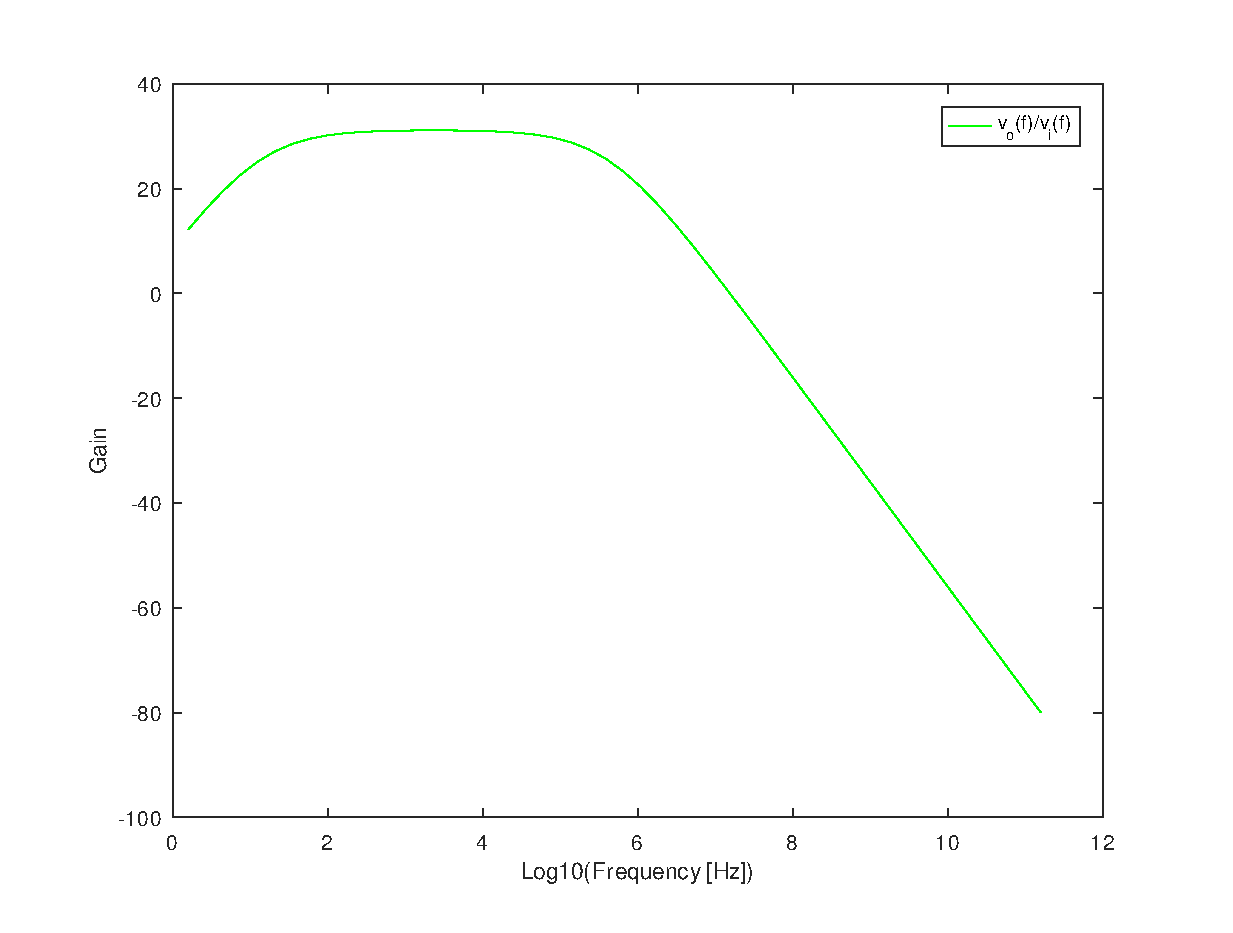
\includegraphics[width = 8cm]{Gain.eps} 
\caption{Gain}
\label{gain}
\end{figure}

By analysing the figure \ref{gain}, we can see that there are 3 types of elements: a NPN BJT, resistors and capacitors.
The first capacitor, $C_in$ , is a coupling capacitor, that acts as a DC Block, so that $V_in$ doesn’t
introduce a DC component of 0, that would change the Operating Point (OP) of the transistor.
The second capacitor, $C _E$ , acts as a bypass capacitor, for it ensures that for low frequencies
all the current flows through $R_E$, and for high frequencies, it passes through the capacitor.
Generally, the output impedance of this stage is high, when compared with the load,
being this the major reason why we cant use just this stage, and we need another one. \par
Both of the capacitors are being analysed in the section of Simulation Analysis.


\subsubsection{Inspection analysis}






\subsubsection{Cutoff frequencies}


\subsection{Output stage}

As we could see in the section of the Gain stage, we end up with a high output impedance $Z_O1$ . For that reason, we
connect a second circuit to the output of the Gain Stage, that produce a low output impedance.
This part of the stage is presented in the figure below:

%\begin{figure}[H] 
%\centering
%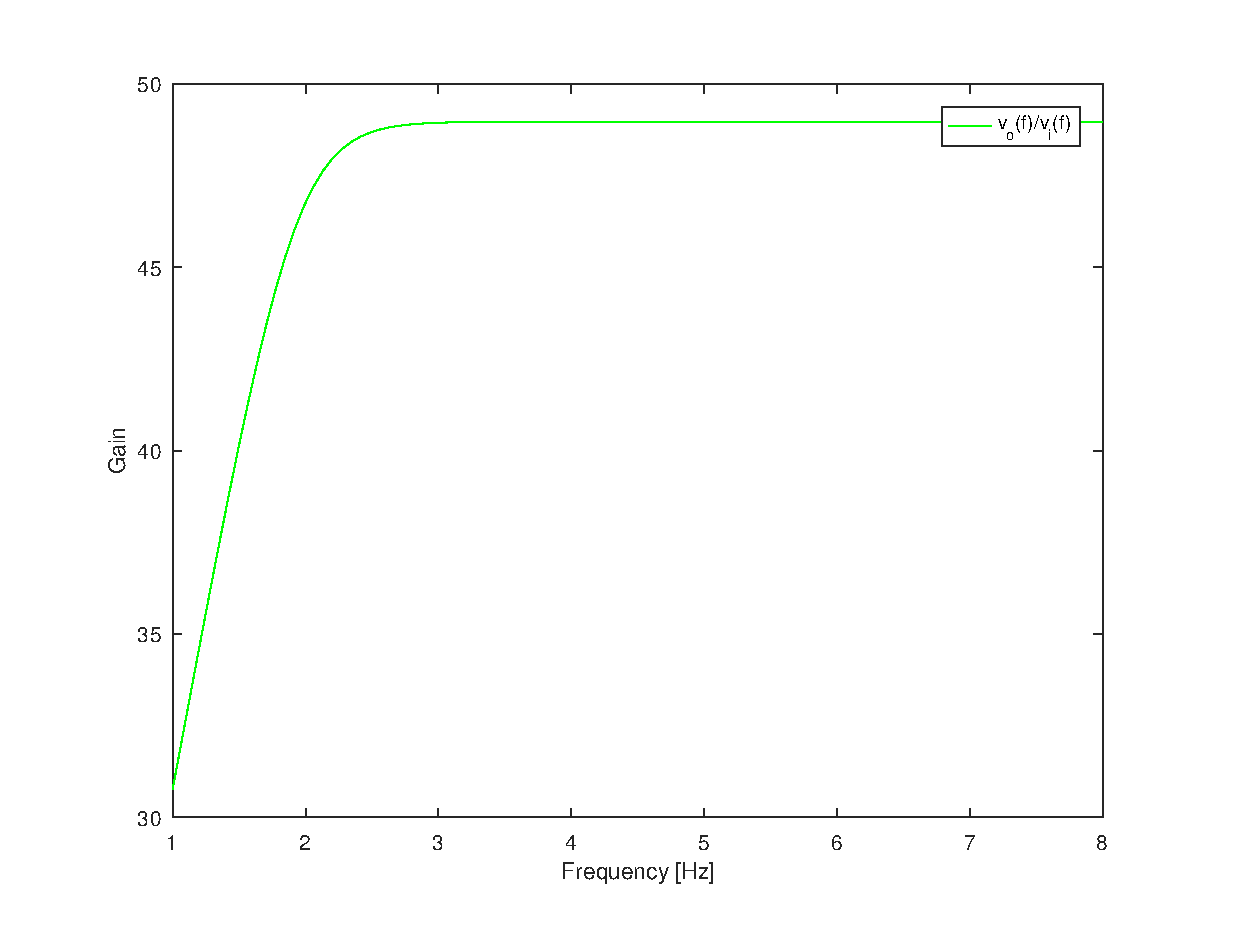
\includegraphics[width = 8cm]{Output.eps} 
%\caption{Output}
%\label{output}
%\end{figure}

By analysing the figure, we can conclude that this circuit presents similar components but with some differences.
Instead of a NPN BJT, we use a PNP BJT, because it has a higher $\beta_F$, that lowers the
output impedance as we desire. It also illustrates the use of another BJT transistor. \par
Another capacitor, $C_o$ , is used with a similar goal as the previous coupling capacitor. If we
didn’t use this component, the gain stage would introduce a DC voltage of 0 to the second stage,
which as previous would change and ruin the transistor’s Operating Point. \par
We will end up with a lower output impedance in this stage, when compared to
the load, and a higher input impedance when compared to the output impedance of the gain
stage. When we combine both stages, we need to ensure that there is a compatibility between the
impedances of both stages. In fact, by the voltage divider law, to make sure no voltage signal is lost, the input
impedance of the second stage should be much greater than the output impedance of the first
one.\par
To conclude, when we merge these two circuits, we end up with the BJT Audio Amplifier represented in Figure 1.

%\begin{table}[H] \centering
%\begin{tabular}{|
%>{\columncolor[HTML]{FFCC67}}l |c|}
%\hline
%\multicolumn{2}{|l|}{\cellcolor[HTML]{EABD8B}Name - Value} \\ \hline
%VCE & 3.363884e+00 V\\ \hline
VBEON & 7.000000e-01 V \\ \hline
VEC & 4.420697e+00 V\\ \hline
VEBON & 7.000000e-01 V \\ \hline
IB1 & 1.103113e-05 A \\ \hline
IC1 & 1.971263e-03 A \\ \hline
IE1 & 1.982294e-03 A \\ \hline
IB2 & -7.377528e-05 A \\ \hline
IC2 & 1.676912e-02 A \\ \hline
IE2 & 1.684290e-02 A \\ \hline

%\end{tabular}
%\caption{optab}
%\end{table}

%\begin{table}[H] \centering
%\begin{tabular}{|
%>{\columncolor[HTML]{FFCC67}}l |c|}
%\hline
%\multicolumn{2}{|l|}{\cellcolor[HTML]{EABD8B}Name - Value} \\ \hline
%First Stage\\ \hline
AV1-DB & 2.634352e+01 dB\\ \hline
ZI1 & 2.811209e+03 Omega \\ \hline
ZO1 & 3.754073e+03 Omega \\ \hline
Second Stage\\ \hline
AV2-DB & -7.252308e-02 dB\\ \hline
ZI2 & 4.075483e+04 Omega \\ \hline
ZO2 & 1.478440e+00 Omega \\ \hline
Complete\\ \hline
ZO & 1.710806e+01 Omega\\ \hline
AV-DB & 2.593695e+01 dB\\ \hline
Merit & 4.398471e+02 \\ \hline
HighCutOff frequency & 8.304945e+05 Hz\\ \hline
LowCutOff frequency & 2.183854e+01 Hz\\ \hline
Cost & 2.242430e+03 MU's\\ \hline
Bandwidth & 8.304726e+05 rad/s\\ \hline

%\end{tabular}
%\caption{Point 2}
%\end{table}

